\section{Zielsetzung}


\section{Theorie}
\label{sec:Theorie}
\subsection{Allgemeine Theorie zum Reflexklystron}

Das Frequenzspektrum von Mikrowellen erstreckt sich von $\SI{300}{\mega\hertz}$ bis $\SI{300}{\giga\hertz}$.
In diesem Versuch wird zur Umwandlung von elektrischer in Mikrowellenenergie ein Reflexklystron benutzt.
Es handelt sich hierbei um eine Mikrowellenröhre, deren Aufbau in Abbildung \ref{fig:klystron} wiedergegeben ist.

\begin{figure}
  \centering
  \includegraphics[height=8cm]{ressources/theorie.png}
  \caption{Schematischer Aufbau eines Klystrons \cite{skript}.}
  \label{fig:klystron}
\end{figure}

Es besteht hauptsächlich aus einem Glühdrat, einem Hochfrequenzresonator und einem Reflektor; letzterem verdankt es seinen Namen.
Aus dem Glühdrat werden Elektronen emittiert, welche zum Resonator beschleunigt werden.
Durchlaufen die Elektronen nun den Resonator, zwischen dessen Gittern ein Hochfrequenzfeld anliegt, tritt Geschwindigkeitsmodulation auf.
Diese ist in Abbildung \ref{fig:mod} dargestellt.

\begin{figure}
  \centering
  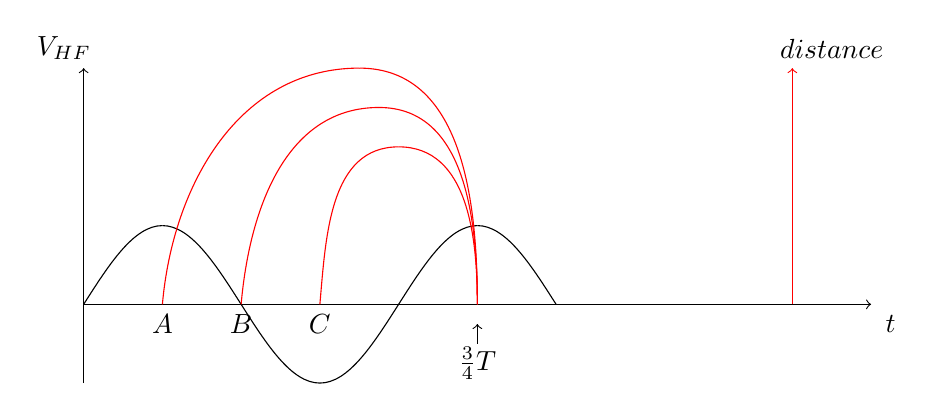
\begin{tikzpicture}
    \draw [->] (0,0) -- (0,4);
    \draw [->] (5,0.5) -- (5,0.75);
    \draw [->] (0,1) -- (10,1);
    \draw [->,red] (9,1) -- (9,4);
    \path node at (-0.25,4.25) {$V_{\text{HF}}$}
          node at (10.25,0.75) {$t$}
          node at (9.5,4.25)  {$\text{distance}$}
          node at (5,0.25) {$\frac{3}{4}T$};
    \draw (0,1) sin (1,2);
    \draw (1,2) cos (2,1);
    \draw (2,1) sin (3,0);
    \draw (3,0) cos (4,1);
    \draw (4,1) sin (5,2);
    \draw (5,2) cos (6,1);
    \path node at (1,0.75) {$A$}
          node at (2,0.75) {$B$}
          node at (3,0.75) {$C$};
    \draw [red] (1,1) to[out=85,in=180] (3.5,4);
    \draw [red] (3.5,4) to[out=0,in=90] (5,1);
    \draw [red] (2,1) to[out=85,in=180] (3.75,3.5);
    \draw [red] (3.75,3.5) to[out=0,in=90] (5,1);
    \draw [red] (3,1) to[out=85,in=180] (4,3);
    \draw [red] (4,3) to[out=0,in=90] (5,1);
  \end{tikzpicture}
  \caption{Darstellung der Geschwindigkeitsmodulation.}
  \label{fig:mod}
\end{figure}

Elektronen, die zu einem früheren Zeitpunkt $A$ in das Hochfrequenzfeld eintreten, werden zusätzlich beschleunigt, wohingegen, welche die zu einem späteren Zeitpunkt $B$ kommen, verlangsamt werden.
Nach passieren des Resonators werden die Elektronen am negativ geladenen Reflektor reflektiert und, bei richtig eingestellter Reflektorspannung, gelangen alle Elektronen zu dem selben Zeitpunkt wieder im Resonator an (bunching), an dem sie maximal abgebremst werden.
Dies findet immer bei $(n+3/4)$ der Periodendauer des Resonators statt.
Die maximale Abbremsung gewährleistet die effektivste Umwandlung in Strahlungsenergie, welche sich im Output wiederspiegelt.\\
Wird die Reflektorspannung nun durchmoduliert, ergibt sich der Zusammenhang von Frequenz und Output, wie er in Abbildung \ref{fig:output} zu sehen ist.

\begin{figure}
  \centering
  \includegraphics[height=6cm]{ressources/output.png}
  \caption{Typisches Signalbild des Versuchs \cite{skript}.}
  \label{fig:output}
\end{figure}

Es sind immer dann Peaks zu sehen, wenn die Reflektorspannung gerade so eingestellt ist, dass ein Elektronenbunch zum Zeitpunkt maximaler Abbremsung in den Resonator zurückkommt.
Ein Peak entspricht dabei einem Modus, welcher durch $(n+3/4)T$, der Aufenthaltsdauer der Elektronen im Resonatorraum, definiert ist.

\subsection{Wellen in einem Hohlleiter}





\cite{sample}

% 2x2 Plot
% \begin{figure*}
%     \centering
%     \begin{subfigure}[b]{0.475\textwidth}
%         \centering
%         \includegraphics[width=\textwidth]{Abbildungen/Schaltung1.pdf}
%         \caption[]%
%         {{\small Schaltung 1.}}
%         \label{fig:Schaltung1}
%     \end{subfigure}
%     \hfill
%     \begin{subfigure}[b]{0.475\textwidth}
%         \centering
%         \includegraphics[width=\textwidth]{Abbildungen/Schaltung2.pdf}
%         \caption[]%
%         {{\small Schaltung 2.}}
%         \label{fig:Schaltung2}
%     \end{subfigure}
%     \vskip\baselineskip
%     \begin{subfigure}[b]{0.475\textwidth}
%         \centering
%         \includegraphics[width=\textwidth]{Abbildungen/Schaltung4.pdf}    % Zahlen vertauscht ... -.-
%         \caption[]%
%         {{\small Schaltung 3.}}
%         \label{fig:Schaltung3}
%     \end{subfigure}
%     \quad
%     \begin{subfigure}[b]{0.475\textwidth}
%         \centering
%         \includegraphics[width=\textwidth]{Abbildungen/Schaltung3.pdf}
%         \caption[]%
%         {{\small Schaltung 4.}}
%         \label{fig:Schaltung4}
%     \end{subfigure}
%     \caption[]
%     {Ersatzschaltbilder der verschiedenen Teilaufgaben.}
%     \label{fig:Schaltungen}
% \end{figure*}
